% The Clever Algorithms Project: http://www.CleverAlgorithms.com
% (c) Copyright 2011 Jason Brownlee. Some Rights Reserved. 
% This work is licensed under a Creative Commons Attribution-Noncommercial-Share Alike 2.5 Australia License.

% Name
% The algorithm name defines the canonical name used to refer to the technique, in addition to common aliases, abbreviations, and acronyms. The name is used in terms of the heading and sub-headings of an algorithm description.
\section{Least Absolute Shrinkage and Selection Operator} 
\label{sec:lasso}
\index{LASSO}
\index{Least Absolute Shrinkage and Selection Operator}
\index{Penalized $L_1$ Regression}
\index{Basis Pursuit}

% other names
% What is the canonical name and common aliases for a technique?
% What are the common abbreviations and acronyms for a technique?
\emph{Least Absolute Shrinkage and Selection Operator, LASSO, Penalized $L_1$ Regression, Basis Pursuit}

% Taxonomy: Lineage and locality
% The algorithm taxonomy defines where a techniques fits into the field, both the specific subfields of Computational Intelligence and Biologically Inspired Computation as well as the broader field of Artificial Intelligence. The taxonomy also provides a context for determining the relation- ships between algorithms. The taxonomy may be described in terms of a series of relationship statements or pictorially as a venn diagram or a graph with hierarchical structure.
\subsection{Taxonomy}
% To what fields of study does a technique belong?
LASSO is a Regularization method for Multiple Linear Regression models, and can be generalized to other machine learning methods.
LASSO may be considered the application of the Basis Pursuit method from Signal Processing to regression.
% What are the closely related approaches to a technique?
LASSO is related to other Regularized methods such as Ridge Regression and Bridge Regression.

% solutions
Solutions to the optimization problem presented by the LASSO method include Least Angle Regression (LARS) and Cyclical Coordinate Descent.
% extensions
Extensions of LASSO include Group LASSO, Blockwise Sparse Regression (BSR), Fused LASSO, Graphical LASSO and the Elastic Net.

% Strategy: Problem solving plan
% The strategy is an abstract description of the computational model. The strategy describes the information processing actions a technique shall take in order to achieve an objective. The strategy provides a logical separation between a computational realization (procedure) and a analogous system (metaphor). A given problem solving strategy may be realized as one of a number specific algorithms or problem solving systems. The strategy description is textual using information processing and algorithmic terminology.
\subsection{Strategy}
% What is the information processing objective of a technique?
The information processing objective of the LASSO is to reduce or shrink the magnitude of the coefficients in a regression model.
% What is a techniques plan of action?
This is achieved by penalizing models based on the sum of the sum of the absolute values of the coefficients being less than a constant parameter ($t$). This penalization of the model is called an $L_1$-penalty or the $L1$-norm penalty of the coefficient vector. This constraint both shrinks the value of coefficients and allows some coefficients to be come exactly zero (unlike Ridge Regression). The effect is that this modification of least squares regression performs both continuous shrinkage of coefficients and automatic selection of variables simultaneously. 

% what is the algorithm where does optimization fit in?
The LASSO methods involves setting all coefficients to zero initially, selecting the most correlated variables and incrementing their coefficients in the direction of their correlation until another variable is as correlated with the residual. The procedure involves building up a set of ``most correlated'' variables with coefficients.

The objective function for the LASSO is non-differentiable and has been subject to intensive research. Tibshirani approached the problem as a quadratic programming problem with linear inequality constraints, where $t$ controls the amount of shrinkage applied to the coefficients \cite{Tibshirani1996} (section 6).


% Heuristics: Usage guidelines
% The heuristics element describe the commonsense, best practice, and demonstrated rules for applying and configuring a parameterized algorithm. The heuristics relate to the technical details of the techniques procedure and data structures for general classes of application (neither specific implementations not specific problem instances). The heuristics are described textually, such as a series of guidelines in a bullet-point structure.
\subsection{Heuristics}
% What are the suggested configurations for a technique?
% What are the guidelines for the application of a technique to a problem instance?

\begin{itemize}
	\item The penalty term $t \geq 0$ controls the amount of shrinkage applied to the model coefficients. If $t$ is too large, then the penalty does not have an effect on the model, as such smaller values are used.
	\item Tibshirani \cite{Tibshirani1996} (section 4) provide three data-based methods for approximating an optimal $t$ value using cross-validation, generalized cross validation and analytics unbiased estimate of risk. Cross-validation is a common method for finding good approximations for the penalty term $t$.
	\item Popular efficient algorithms for solving the LASSO method include Least Angle Regression (LARS) \cite{Efron2002} and Coordinate Descent \cite{Friedman2007}.
	\item It has been shown to achieve some of the benefits of both Subset Selection (feature selection) and Ridge Regression (shrinkage of coefficients).
	\item The penalization scheme is general and can be applied to models beyond regression.
	\item The sparse model representation achieved by the LASSO can lead to simpler models that are easier to interpret. 
	\item It is most suited for datasets where there are are a large number of small effects and least suited to problems where there are a small number of large effects.
	\item It provides sparse solutions in problems where the number of predictors $p$ is larger than the number of observed cases $n$ ($p>n$ problems).
	\item Zou and Hastie describe three limitations of the LASSO: a) in $p>n$ problems (more variables than observations) the LASSO is limited to selecting $n$ variables, b) it selects one variable from the group of variables that pairwise highly-correlated, c) it is outperformed by ridge regression when there is high correlation between variables \cite{Zou2005}.
\end{itemize}

% sample script in R
\subsection{Code Listing}
% listing
Listing~\ref{lars_lasso_regression} provides a code listing of the LASSO method in R.
% algorithm and package
The example uses the \texttt{lars()} function in the \texttt{lars} core package. The \texttt{lars} package provides the Least Angle Regression, Lasso, Stepwise Regression and the Forward Stagewise algorithms for regularization \cite{Hastie2011}. 

% what is the optimization procedure?
The \texttt{lars()} function uses the Least Angle Regression algorithm to solve the LASSO, computing a LASSO solution for all values of the shrinkage or penalty parameter ($t$) simultaneously in the same computational cost as a least squares fit.
% what is the estimation of t?
The implementation works by starting at $t=0$ and adding the most correlated values and increasing coefficients in the direction of the correlations as $t$ is increased. Coefficients for a given $t$ value can then be selected using a measure of model error, such as Sum Squared Residual error.
For more information on the algorithm used by the implementation, refer to Efron et~al.\ \cite{Efron2002}.

Figure~\ref{plot:lasso_result} provides a plot of the coefficient values of each model for the given $t$ value. This is called a solution path graph or a plot of solution paths for coefficients and can aid in understanding in the selection of suitable $t$ values and in turn suitable model coefficients. For more information on this library type: \texttt{library(help="lars")}, and for more information on the function type: \texttt{?lars}.

% problem
The test problem is a four-dimensional dataset of 100 samples, where \texttt{x3} and \texttt{y} are dependent on \texttt{x1} and \texttt{x1} and \texttt{x2} are independent variables. The problem is ill defined as \texttt{y} given \texttt{x1, x2, x3}. The model is expected to reduce the contribution of \texttt{x2} and \texttt{x3} toward zero leaving \texttt{y} given \texttt{x1}.

% TODO provide a better problem with real variable selection

% example
The example shows the preparation of a model using LASSO with the LARS solution. The step in the resulting model with the minimum Sum Squared Residual error is selected. The names of the variables in the selected model are displayed and the selected model is used to make predictions.

\lstinputlisting[firstline=7,language=r,caption={Example of LASSO in R using the \texttt{lars()} function in the \texttt{lars} package.}, label=lars_lasso_regression]{../src/algorithms/regularization/lars_lasso_regression.R}

\begin{figure}[htp]
\centering
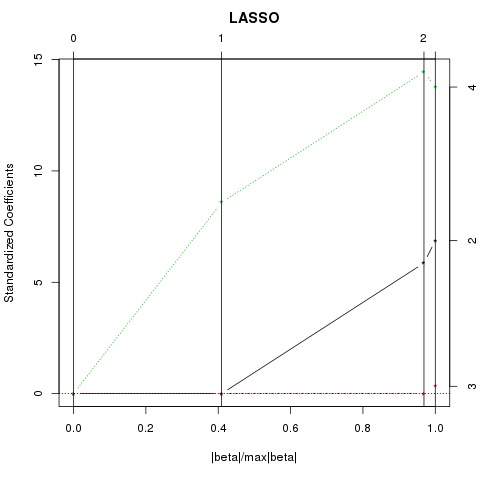
\includegraphics[scale=0.60]{a_regularization/lasso_result.png}
\caption{Graph of solution paths for LASSO.}
\label{plot:lasso_result}
\end{figure}

% other packages
Other packages provide implementations of the Lasso penalty method.
The \texttt{glmnet} package provides the LASSO and Elastic Net regularization for Generalized Linear Models (GLMs) using Coordinate Descent \cite{Friedman2011}.
The \texttt{grplasso} package provides an the Group Lasso penalty method for fitting models \cite{Meier2009}.
The \texttt{grpreg} package provides lasso regularization with grouped covariates \cite{Brehen2011}.

% lmmlasso package?!?
% penalized package

% References: Deeper understanding
% The references element description includes a listing of both primary sources of information about the technique as well as useful introductory sources for novices to gain a deeper understanding of the theory and application of the technique. The description consists of hand-selected reference material including books, peer reviewed conference papers, journal articles, and potentially websites. A bullet-pointed structure is suggested.
\subsection{References}
% What are the primary sources for a technique?
% What are the suggested reference sources for learning more about a technique?

% primary sources
\subsubsection{Primary Sources}
% primary
The LASSO method was described in detail by Tibshirani who also provided a Bayes model for the LASSO, simulation studies and extensions to generalization regression and other problems \cite{Tibshirani1996}. Tibshirani attributes the motivation the LASSO to Breiman's Non-negative Garrotte regression method \cite{Breiman1993} (later published \cite{Breiman1995}).
The LASSO is equivalent to Basis Pursuit from the field of Signal Processing \cite{Chen1998}.

% more info
\subsubsection{More Information}
The focus of the research into the LASSO is on efficient algorithms for solving the objective function.
% lars
Efron et~al.\ developed an efficient algorithm for computing the entire regularization path for the LASSO called Least Angle Regression (LARS) \cite{Efron2002}. LARS is based on the Homotopy method described by Osborne et~al.\ \cite{Osborne2000}. LARS has the same computational cost as the full least-squares fit on the data, exploiting the fact the coefficient profiles are piecewise linear.

% coordinate descent
Many solutions to the LASSO method have been proposed that optimize one parameter (coordinate) at a time, so called path-wise or coordinate-wise optimization methods. Early attempts were made by Fu in an investigation of cyclic coordinate descent for $L_2$ regression \cite{Fu1998} and Daubechies et~al.\ \cite{Daubechies2004}. The approach was re-discovered and promoted as an competitive and simpler alternative to LARS by Friedman et~al.\ for LASSO and related regularization methods with linearly-separable coefficients \cite{Friedman2007}. Wu and Lange provide a in-depth study of coordinate descent algorithms for LASSO penalized regression \cite{Wu2008}.

% extensions
There are many extensions to the LASSO method.
Graphical LASSO is an application of the method to undirected graphical models \cite{Friedman2008a}.
Fused LASSO the penalizes the $L_1$-norm of both the coefficients and their successive differences suitable for problems with features that can be ordered \cite{Tibshirani2005}.
Group LASSO \cite{Yuan2006} and Blockwise Sparse Regression (BSR) \cite{Kim2006} are extensions of the LASSO method for finding sparse groups (block-wise sparsity) of variables.
Zou and Hastie describe the Elastic Net which combines the $L_1$-penalty of LASSO with the $L_2$-penalty of Ridge Regression and provide a LARS-based solution \cite{Zou2005}.


% END